% !TEX TS-program = pdflatexmk

\documentclass[12pt,compress]{beamer}
\usepackage{newtxtext,newtxmath}
\usepackage[utf8]{inputenc}
\usepackage{microtype}
\usepackage{array}
\usepackage{hyperref}
\usepackage{graphicx}
\usepackage{setspace}
\usepackage{tikz}
\usetikzlibrary{shapes.multipart}
\usetikzlibrary{positioning}
\usetikzlibrary{arrows}
\usepackage{pgfplots}
\pgfplotsset{compat=1.7}
\usepackage{forest}
\useforestlibrary{linguistics}
\usepackage{appendixnumberbeamer}
\usepackage[style=authoryear,uniquename=false,maxnames=2,minnames=1,maxbibnames=99,sorting=nyt,backend=biber]{biblatex}
\AtEveryBibitem{\clearfield{note}}


\addbibresource{bethard.bib}
\addbibresource{extra.bib}
\renewcommand*{\bibfont}{\scriptsize}

% Define UA colors
% https://brand.arizona.edu/guide/color
\definecolor{ua-red}{HTML}{AB0520}
\definecolor{ua-blue}{HTML}{0C234B}

\colorlet{event}{ua-red}
\colorlet{time}{ua-blue}
\colorlet{partialtime}{time!50!white}
\tikzset{
  relation-type/.style={auto, font=\scriptsize\scshape},
  relation-path/.style={thick, ->},
  on/.code n args={2}{\alt<#1>{\pgfkeysalso{#2}}{}},
  annotate on/.code n args={2}{\alt<#1>{}{\pgfkeysalso{opacity=0, every #2 node part/.style={text opacity=1}}}},
}
\setlength\fboxrule{1pt}
\setlength\fboxsep{1pt}
\newcommand{\eventbox}[1]{\fcolorbox{event}{white}{#1}}
\newcommand{\timebox}[1]{\fcolorbox{time}{white}{#1}}
\newcommand{\smallcite}[1]{{\scriptsize\parencite{#1}}}
\newcommand{\nonterm}[1]{\textsc{[#1]}}
\newcommand{\word}[1]{\textit{#1}}
\newcommand{\operator}[1]{\textsc{#1}}

% smaller than \strut, but ensures a constant height
\newcommand{\fullheight}{\vphantom{(p}}

% command for annotating words in text
% #1: drawing options
% #2: name of entire shape
% #3: number of parts
% #4: name of baseline part
% #5: annotation type
% #6: node text following \nodepart{two}
\newcommand{\annotate}[6][]{%
\tikz[remember picture,baseline={(#2.#4)}]{%
\node[
  rectangle split,
  rectangle split parts=#3,
  thick,
  inner sep=2pt,
  align=center,
  draw=event,
  #1]%
(#2)
{%
\scriptsize\fullheight\textsc{#5}%
\nodepart{two}%
#6%
\fullheight};}}

% short commands for annotations of various sizes
\newcommand{\AnnotateTwo}[4][]{\annotate[#1]{#2}{2}{two}{#3}{#4}}
\newcommand{\AnnotateThree}[5][]{\annotate[#1]{#2}{3}{three}{#3}{%
\scriptsize\fullheight\textsc{#4}%
\nodepart{three}%
#5}}
\newcommand{\AnnotateFour}[6][]{\annotate[#1]{#2}{4}{four}{#3}{%
\scriptsize\fullheight\textsc{#4}%
\nodepart{three}%
\scriptsize\fullheight\textsc{#5}%
\nodepart{four}%
#6}}
\newcommand{\AnnotateFive}[7][]{\annotate[#1]{#2}{5}{five}{#3}{%
\scriptsize\fullheight\textsc{#4}%
\nodepart{three}%
\scriptsize\fullheight\textsc{#5}%
\nodepart{four}%
\scriptsize\fullheight\textsc{#6}%
\nodepart{five}%
#7}}
\newcommand{\AnnotateSix}[8][]{\annotate[#1]{#2}{6}{six}{#3}{%
\scriptsize\fullheight\textsc{#4}%
\nodepart{three}%
\scriptsize\fullheight\textsc{#5}%
\nodepart{four}%
\scriptsize\fullheight\textsc{#6}%
\nodepart{five}%
\scriptsize\fullheight\textsc{#7}%
\nodepart{six}%
#8}}

% short commands for animated annotations of various sizes
\newcommand{\AnnotateTwoOn}[5][]{\annotate[#1,annotate on={#2}{two}]{#3}{2}{two}{#4}{#5}}

% command for adding links
% #1: drawing options (typically, the color)
% #2: edge options (typically out=NN, in=NN)
% #3: start anchor for arrow
% #4: end anchor for arrow
\newcommand{\AnnotateLink}[4][]{%
\path[color=time,thick,->,#1] (#3) node [circle,color=time,fill,inner sep=0.25ex,#1] {} edge[#2] (#4);}


% command for drawing a timeline
% #1: drawing options
% #2: number of primary intervals
% #3: number of secondary intervals per primary interval
\newcommand{\tikztimeline}[3][]{%
\pgfmathsetmacro{\primaryend}{#2-1}
\pgfmathsetmacro{\secondaryend}{#3-1}
% horizontal line
\draw[#1,dashed] (-0.33,0) -- (0,0);
\draw[#1] (0,0) -- (#2,0);
\draw[#1,dashed,-latex] (#2,0) -- (#2 + 0.33,0);
% primary ticks
\foreach \primary  in {0,...,\primaryend} {%
  \draw[#1] (\primary,0) -- (\primary,\normalbaselineskip);
  % secondary ticks
  \foreach \secondary [evaluate=\secondary] in {\primary+1/#3,\primary+.../#3,\primary+\secondaryend/#3} {
    \draw[#1] (\secondary,0) -- (\secondary,0.5\normalbaselineskip);
  }
}
\draw[#1] (#2,0) -- (#2,\normalbaselineskip);
}

% command for drawing a interval on a timeline
% #1: drawing options
% #2: start time (i.e., start x position)
% #3: end time (i.e., start x position)
% #4: vertical tier (i.e., y position)
% #5: text
\newcommand{\tikztimelineinterval}[5][]{%
\draw[line width=0.9\normalbaselineskip,draw=time,text=white,#1] (#2, #4\normalbaselineskip) -- (#3, #4\normalbaselineskip) node[midway,font=\footnotesize] {#5};
}

% short command for drawing an interval the width of a single primary interval
\newcommand{\tikztimelineprimaryinterval}[4][]{\tikztimelineinterval[#1]{#2}{#2+1}{#3}{#4}}


\mode<presentation>{
\usetheme{Madrid}
\usecolortheme[named=ua-red]{structure}
\setbeamertemplate{navigation symbols}{}
\setbeamertemplate{section in toc}[square]
\setbeamertemplate{subsection in toc}[square]
\setbeamertemplate{items}[square]
\setbeamercovered{invisible}
}

\newcommand{\host}{University of Arizona}
\newcommand{\texttoday}{6 Apr 2018}
\newcommand{\isotoday}{2018-04-06}
\newcommand{\isodaybeforeyesterday}{2018-04-04}
\newcommand{\isoweekofmarchsix}{2018-W10}

\title[\url{http://bethard.faculty.arizona.edu/}]{Teaching Computers the Language of Time}
\author[Dr. Bethard]{Dr. Steven Bethard}
\institute[UA iSchool]{%
School of Information\\
University of Arizona}
\date{\texttoday}

\begin{document}


\section{Motivation}


\begin{frame}[plain]
  \titlepage
\end{frame}


\begin{frame}{An interactive timeline of the Arab Spring}
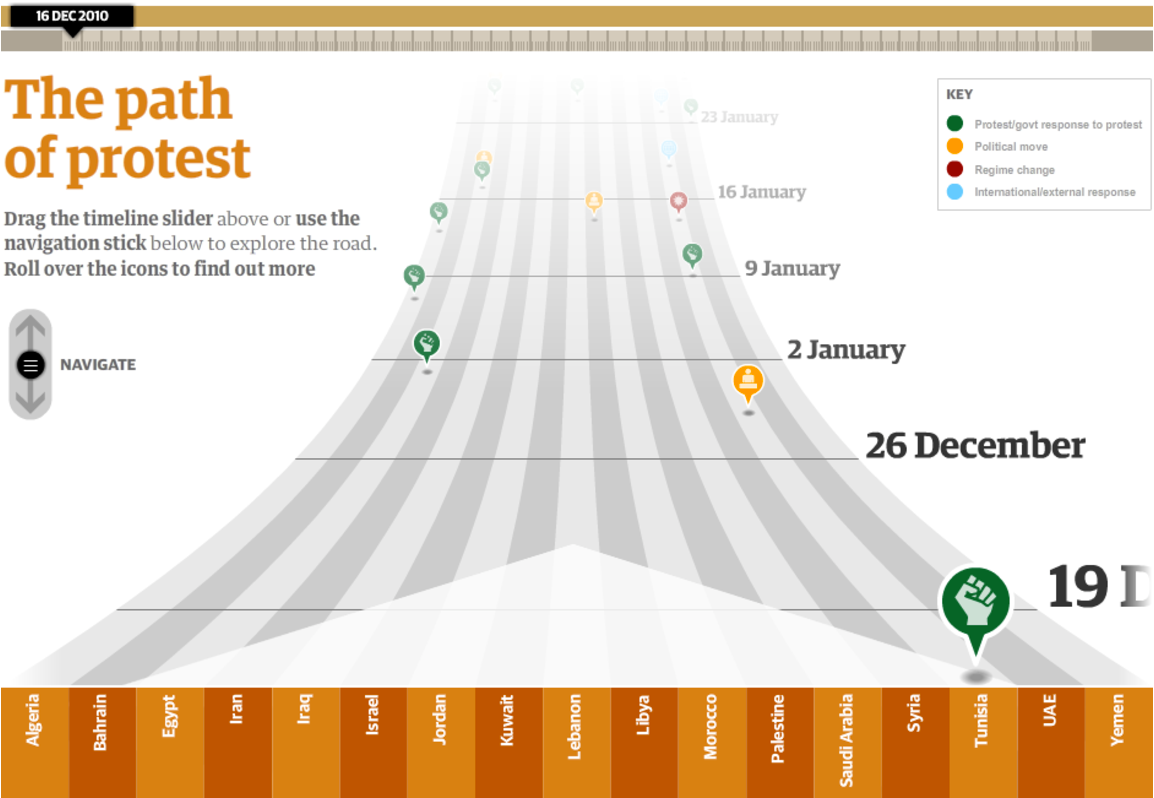
\includegraphics[width=0.9\textwidth]{arab-spring}

{\tiny\url{www.guardian.co.uk/world/interactive/2011/mar/22/middle-east-protest-interactive-timeline}}
\end{frame}


\begin{frame}{An interactive patient timeline}
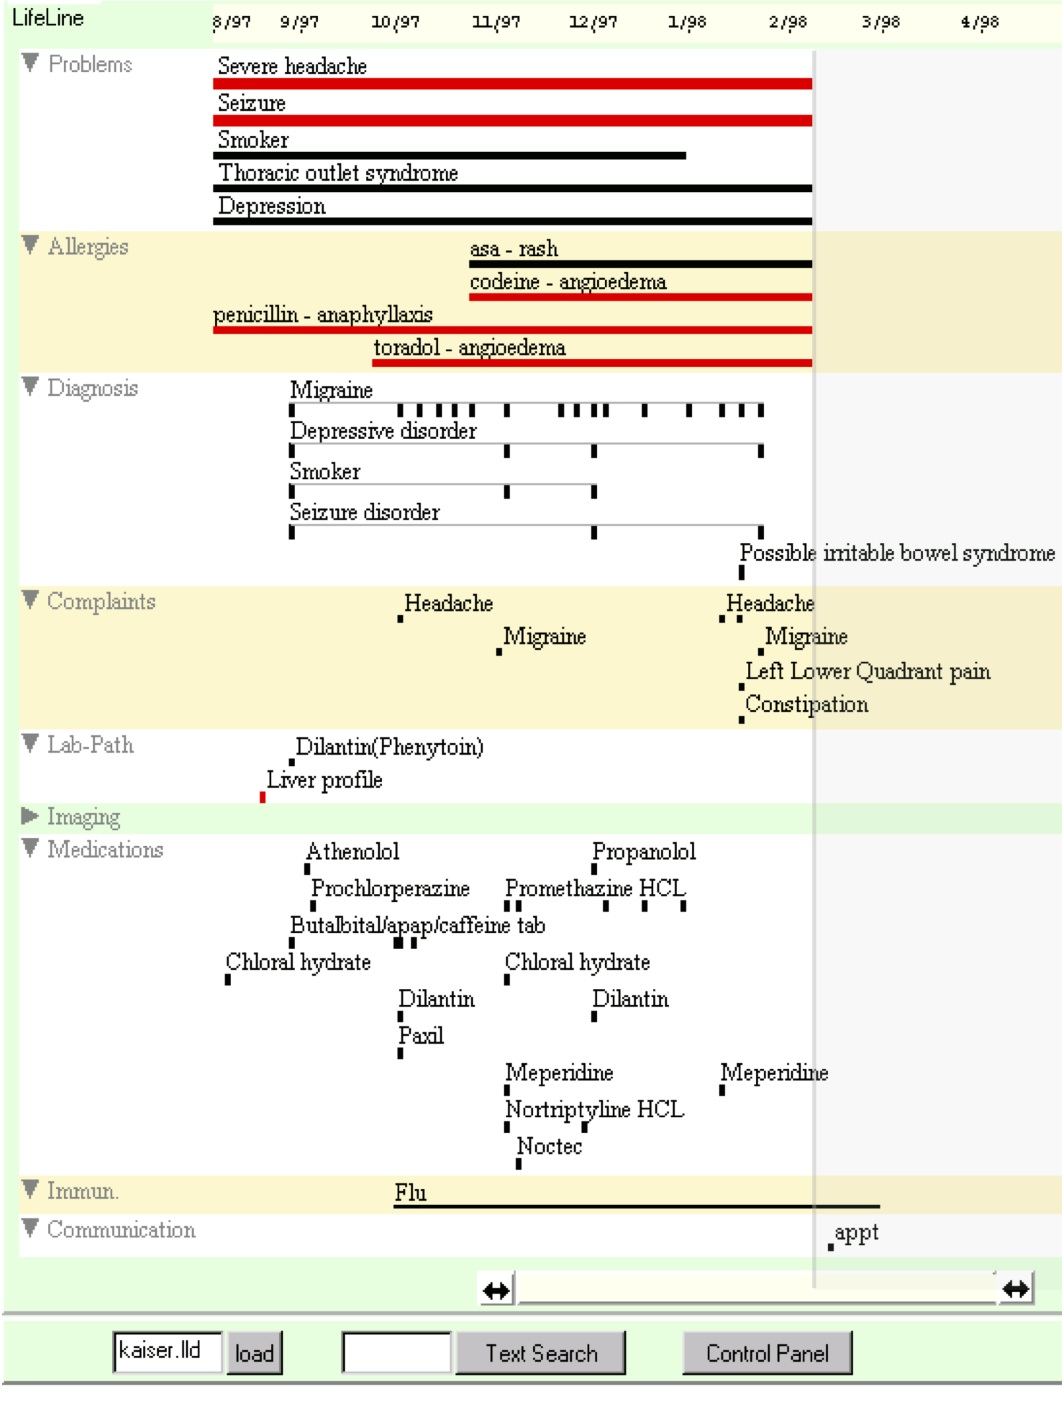
\includegraphics[width=\textwidth,trim={0 5in 0 0},clip]{kaiserlifelines.jpg}
\end{frame}


\begin{frame}{A timeline model should predict like humans}
\begin{tikzpicture}[auto]
\node (text) {\parbox{0.225\textwidth}{\tiny At least 11 people have died in new clashes with security forces in Tunisia after four weeks of unrest, it was reported today.
Rioting against joblessness and other social ills has scarred many cities in the country since 17 December, when a 26-year-old graduate set himself on fire\ldots}};
\node (human) [right=2em of text] {
  \begin{tikzpicture}[auto]
  \node at (0, 1) (1) {
\includegraphics[width=0.2\textwidth]{male-user}};
  \node at (0.5, 0.5) (2) {
\includegraphics[width=0.2\textwidth]{female-user}};
  \end{tikzpicture}
  }
  edge [<-,ultra thick] (text);
\node (model) [right=2em of text,below=of human] {$\text{\LARGE h}\left(\text{\parbox{0.225\textwidth}{\tiny
At least 11 people have died in new clashes with security forces in Tunisia after four weeks of unrest, it was reported today.
Rioting against joblessness and other social ills has scarred many cities in the country since 17 December, when a 26-year-old graduate set himself on fire\ldots
}}\right)$}
  edge [<-,ultra thick] (text);
\node (timeline) [right=2em of human,right=of model] {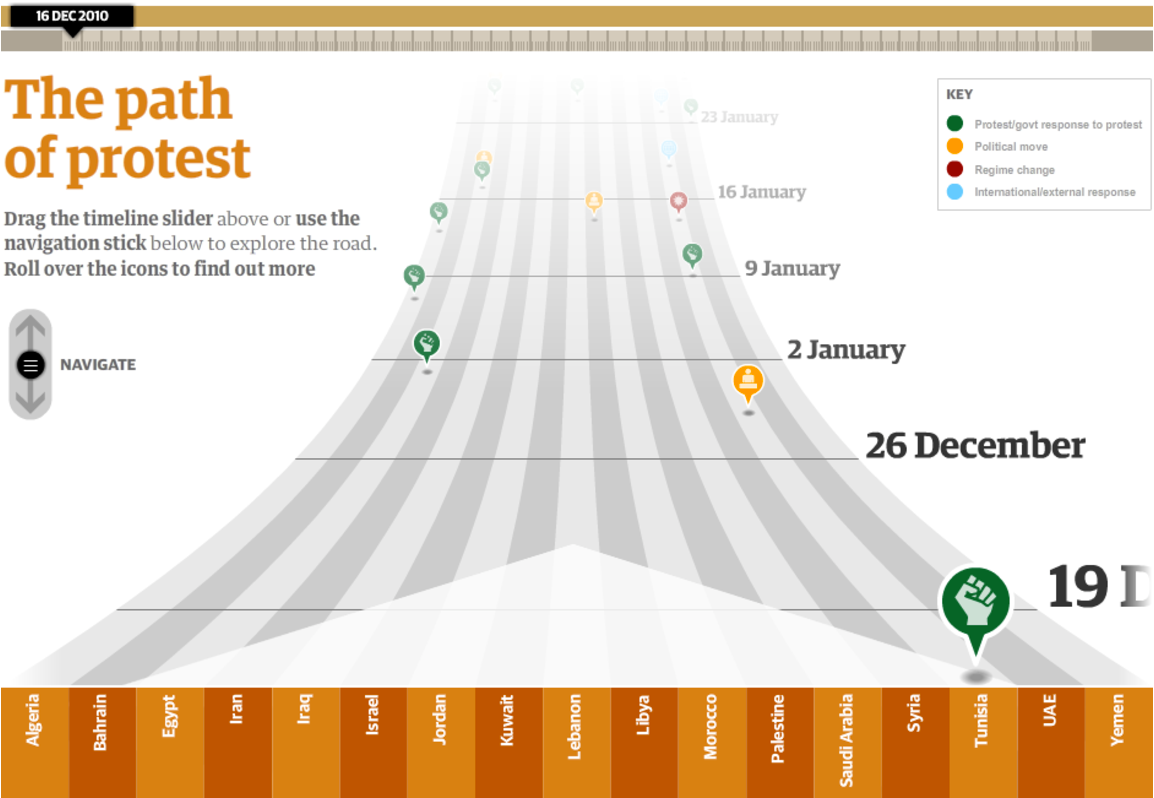
\includegraphics[width=0.25\textwidth]{arab-spring}}
  edge [<-,ultra thick]  (human)
  edge [<-,ultra thick]  (model);
\end{tikzpicture}
\end{frame}


\begin{frame}{Open issues in training a timeline model}
\begin{itemize}[<+->]
\item Translating directly from text to visualization is infeasible
\begin{itemize}
\item What are appropriate intermediate representations?
\end{itemize}
\bigskip
\item Human annotation is needed to provide training examples
\begin{itemize}
\item How do we reliably elicit human understanding of timelines?
\item \textit{Model performance bounded by human agreement}
\end{itemize}
\bigskip
\item Intermediate representations must be (machine) learnable
\begin{itemize}
\item How best can we frame subtasks as machine learning problems?
\end{itemize}
\end{itemize}
\end{frame}


\begin{frame}{Outline}
\tableofcontents
\end{frame}


\AtBeginSection[]
{
 \begin{frame}<beamer>
 \frametitle{Outline}
 \tableofcontents[currentsection]
 \end{frame}
}


\section{Timelines as graphs}


\begin{frame}{Timelines as graphs: ISO-TimeML \smallcite{pustejovsky2010iso}}
\begin{columns}
\begin{column}{0.35\textwidth}
\small
At least 11 people have died in new clashes with security forces in Tunisia after four weeks of unrest, it was reported today.
Rioting against joblessness and other social ills has scarred many cities in the country since 17 December, when a 26-year-old graduate set himself on fire when police confiscated his fruits and vegetables for selling without a permit\ldots
\end{column}
{\Huge $\Rightarrow$}
\begin{column}{0.55\textwidth}
\small
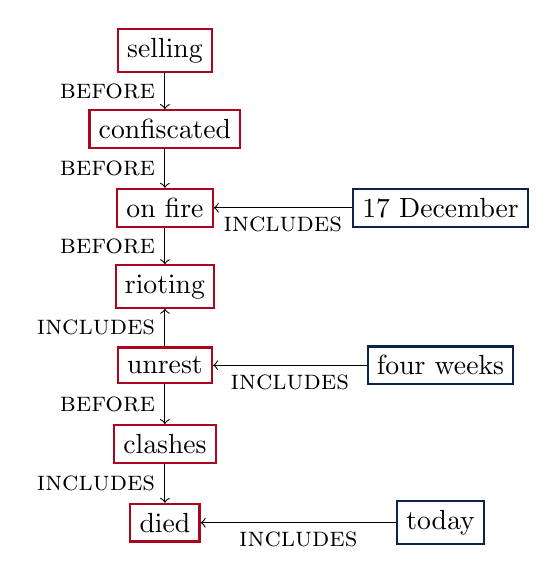
\begin{tikzpicture}[auto]
\node[draw=event,thick] at (0, 6) (selling) {selling};
\node[draw=event,thick] at (0, 5) (confiscated) {confiscated}
  edge [<-] node {\textsc{before}} (selling);
\node[draw=event,thick] at (0, 4) (on fire) {on fire}
  edge [<-] node {\textsc{before}} (confiscated);
\node[draw=time,thick] at (3.5, 4) (17 December) {17 December}
  edge [->] node {\textsc{includes}} (on fire);
\node[draw=event,thick] at (0, 3) (rioting) {rioting}
  edge [<-] node {\textsc{before}} (on fire);
\node[draw=event,thick] at (0, 2) (unrest) {unrest}
  edge [->] node {\textsc{includes}} (rioting);
\node[draw=time,thick] at (3.5, 2) (four weeks) {four weeks}
  edge [->] node {\textsc{includes}} (unrest);
\node[draw=event,thick] at (0, 1) (clashes) {clashes}
  edge [<-] node {\textsc{before}} (unrest);
\node[draw=event,thick] at (0, 0) (died) {died}
  edge [<-] node {\textsc{includes}} (clashes);
\node[draw=time,thick] at (3.5, 0) (today) {today}
  edge [->] node {\textsc{includes}} (died);
\end{tikzpicture}
\end{column}
\end{columns}
\end{frame}


\section{Temporal relations}


\subsection{Annotation paradigms}


\begin{frame}{TimeBank: annotating salient relations}
\end{frame}


\begin{frame}{TempEval: annotating sparse pair-wise relations}
\end{frame}


\begin{frame}{Dense TimeBank: annotating pair-wise relations}
\end{frame}


\begin{frame}{Annotating syntax-driven pair-wise relations}
\end{frame}


\begin{frame}{Annotating relations as tree structures}
\end{frame}


\subsection{Model architectures}


\begin{frame}{Relation detection as all-pairs classification}
\end{frame}


\begin{frame}{Relation detection as parsing}
\end{frame}


\section{Times}


\subsection{Annotation paradigms}


\begin{frame}{TimeBank: annotating flat time expressions}
\end{frame}


\begin{frame}{SCATE: annotating times compositionally}
\end{frame}


\subsection{Model architectures}


\begin{frame}{Time normalization via hand-designed grammars}
\end{frame}


\begin{frame}{Time normalization as parsing}
\end{frame}


\section{Events}


\subsection{Annotation paradigms}


\begin{frame}{TimeBank: events as anything anchored in time}
\end{frame}


\begin{frame}{THYME: events as clinically relevant happenings}
\end{frame}


% include event duration work?


\subsection{Model architectures}

\begin{frame}{Event detection as word classification}
% major performance drop in cross-domain
\end{frame}


\section{Future directions}


\begin{frame}{Summary and future directions}
\end{frame}


\begin{frame}[allowframebreaks]{References}
\printbibliography
\end{frame}


\end{document}
